\section{Metodología aplicada}

En la primera etapa del proyecto se concretaron múltiples reuniones con todos los integrantes del grupo para unificar 
las ideas principales, entre ellas los primeros pasos para comenzar con el diseño de arquitectura, los servicios 
y los repositorios a crear, junto a sus \textit{templates} de directorios y \textit{pipelines} necesarios. En esta etapa 
también se logró estimar las fases del proyecto, como dividir módulos por lógica, features en las fases, y realizar un 
\textit{brainstorming} sobre features obligatorias y secundarias que existirían en la totalidad del proyecto.

\subsection{Herramientas de planificación, visualización y Comunicación}

Para la planificación, visualización y comunicación del proyecto se utilizaron múltiples herramientas:
\vspace{0.25cm}

\textbf{\underline{Miro}}: para la creación y visualización más ``amigable" de las user stories propuestas, creando un 
\textit{User Story Map} (USM) y un \textit{Work Breakdown Structure} (WBS) para realizar un mapeo general, dividirlos 
en módulos/etapas y sea más fácil de explicar al tutor con el fin de exponer la planificación a lo largo del tiempo 
y mostrar las modificaciones si las hubiera. Dentro de estos esquemas lo más utilizado por nosotros y el tutor, fue tener 
un seguimiento de las versiones y su progreso en el tiempo, y poder estimar mejor que features habría que darle más prioridad, 
cuáles se pueden aplazar y cuáles descartar en caso de no llegar para la entrega del producto. Junto a las \textit{User Stories} 
(US) dentro de cada versión, se agregó características con mayor nivel de complejidad que afectan todo o la mayor parte 
del proyecto que son primordiales y deben ser completadas en cada versión, ya que son características troncales y 
requeridas para cumplir los objetivos del proyecto en sí.
\vspace{0.25cm}

\begin{figure}[H]
    \centering
    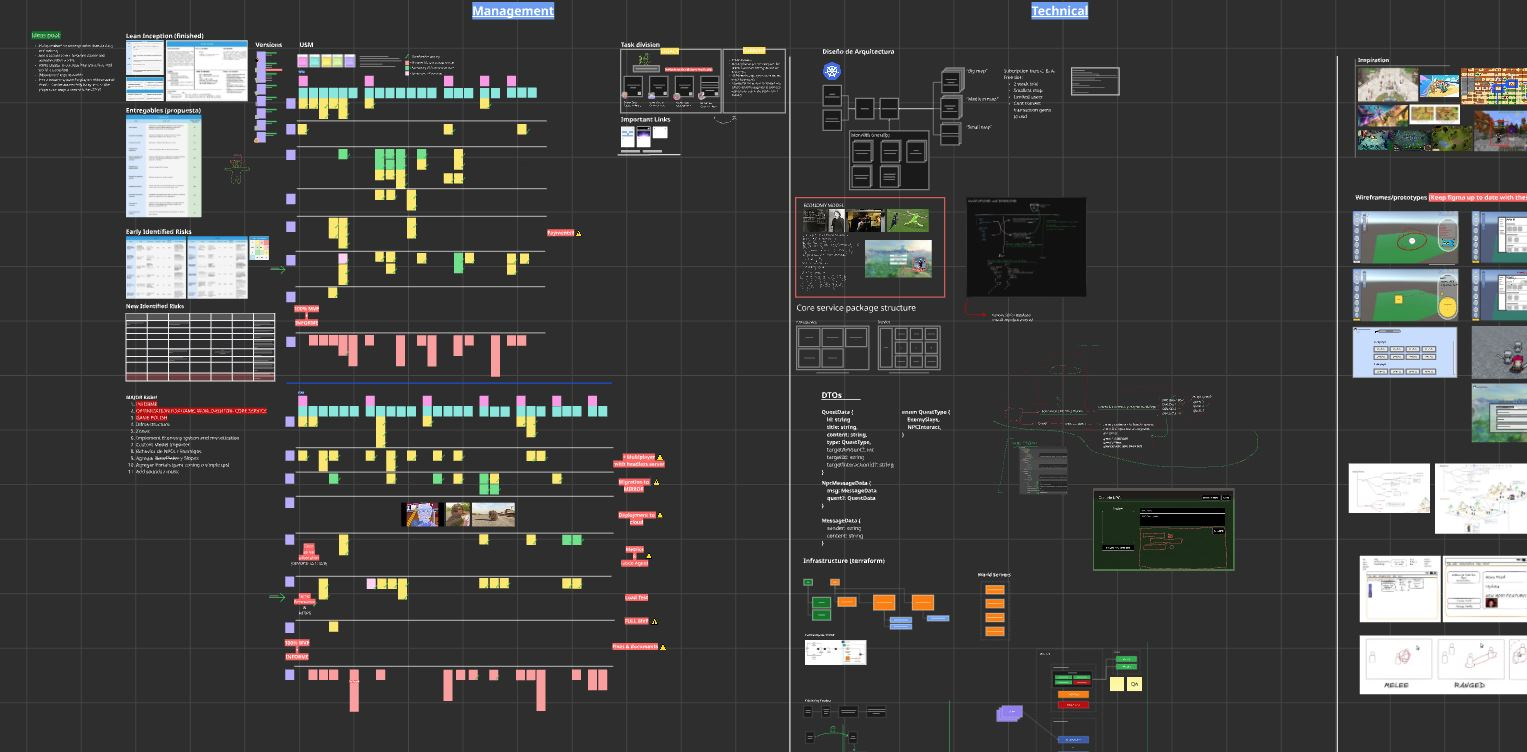
\includegraphics[width=0.85\textwidth]{img/miro.jpg}
    \caption{Captura del Miro utilizado para planificación}
    \label{fig:miro}
\end{figure}

\textbf{\underline{Github projects}}: En la primera etapa del proyecto, una vez que se revisaron y confirmaron la mayoría de las user stories 
entre el grupo y el tutor, se empezó a migrar las mismas user stories del USM diagramado en el Miro. Luego en el comienzo 
de cada iteración, de duración de dos semanas, se revisa que las user stories que deben estar en progreso en esa iteración 
o si existe una siguiente en la misma versión, todas ellas deben tener una estimación aproximada de dificultad, si supera un 
cierto umbral de valor de estimación, debe dividirse en otra/s o en substories.
\vspace{0.25cm}

También se corrobora con consenso grupal cuáles son los criterios de aceptación (CA) utilizando el formato o método 
\textbf{Given-When-Then} para cada user story, para evitar confusiones de nombres similares pero diferentes tareas 
dependiendo del repositorio correspondiente. Cumpliendo lo anterior, si una US no llegó a iniciarse o quedó parcialmente 
completa, en la reunión a fin de iteración se llega a un consenso si debe pasarse a siguiente iteración o almacenarse a 
futuro junto con otras para determinar si entra en el alcance del proyecto.
\vspace{0.25cm}

\begin{figure}[H]
    \centering
    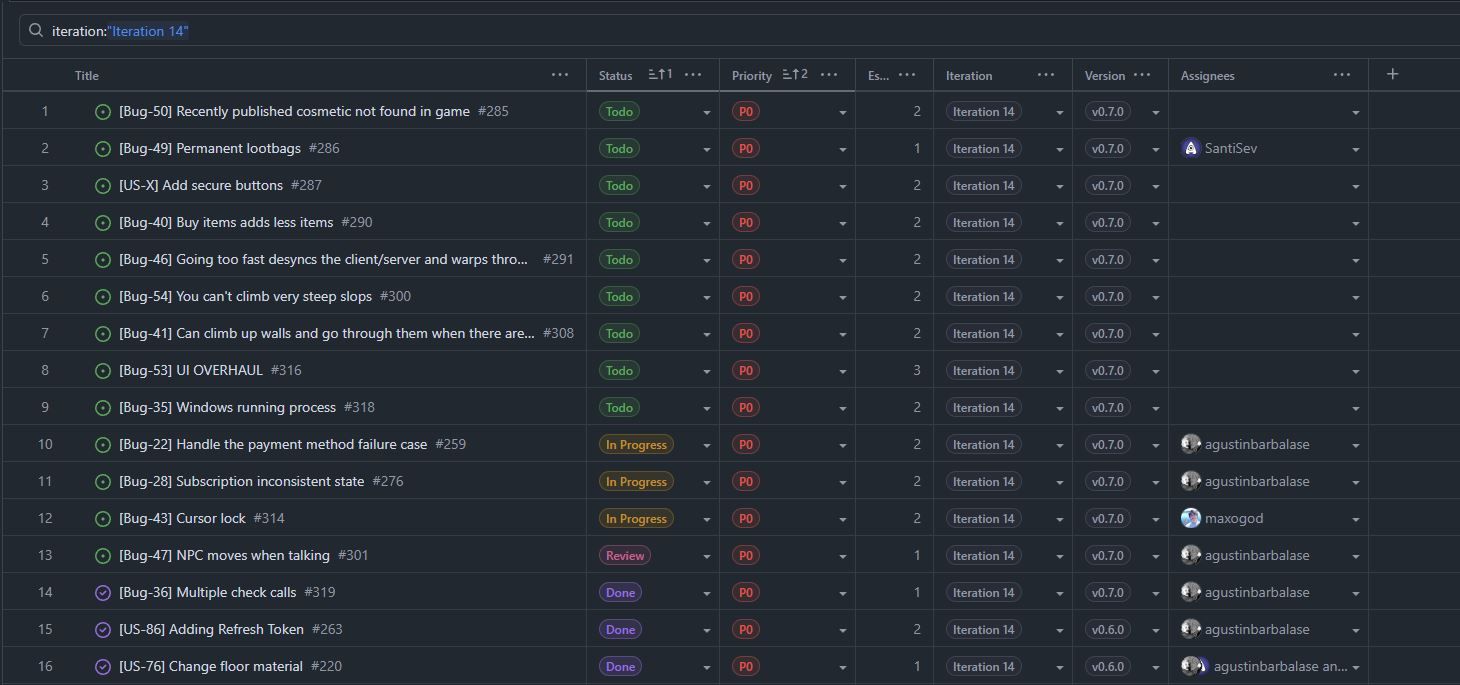
\includegraphics[width=0.85\textwidth]{img/github-projects.jpg}
    \caption{Ejemplo de la organización de las US en Github Projects, con su respectiva prioridad y estado.}
    \label{fig:github-projects}
\end{figure}

\textbf{\underline{Excalidraw}}: para realizar esquemas, croquis, posibles diseños de UI y diagramas de funcionamiento 
del flujo de sistemas más complejos. Algunos son públicos para complementar la documentación y otros son privados con el 
fin de visualizar ideas entre los integrantes.
\vspace{0.25cm}

\begin{figure}[H]
    \centering
    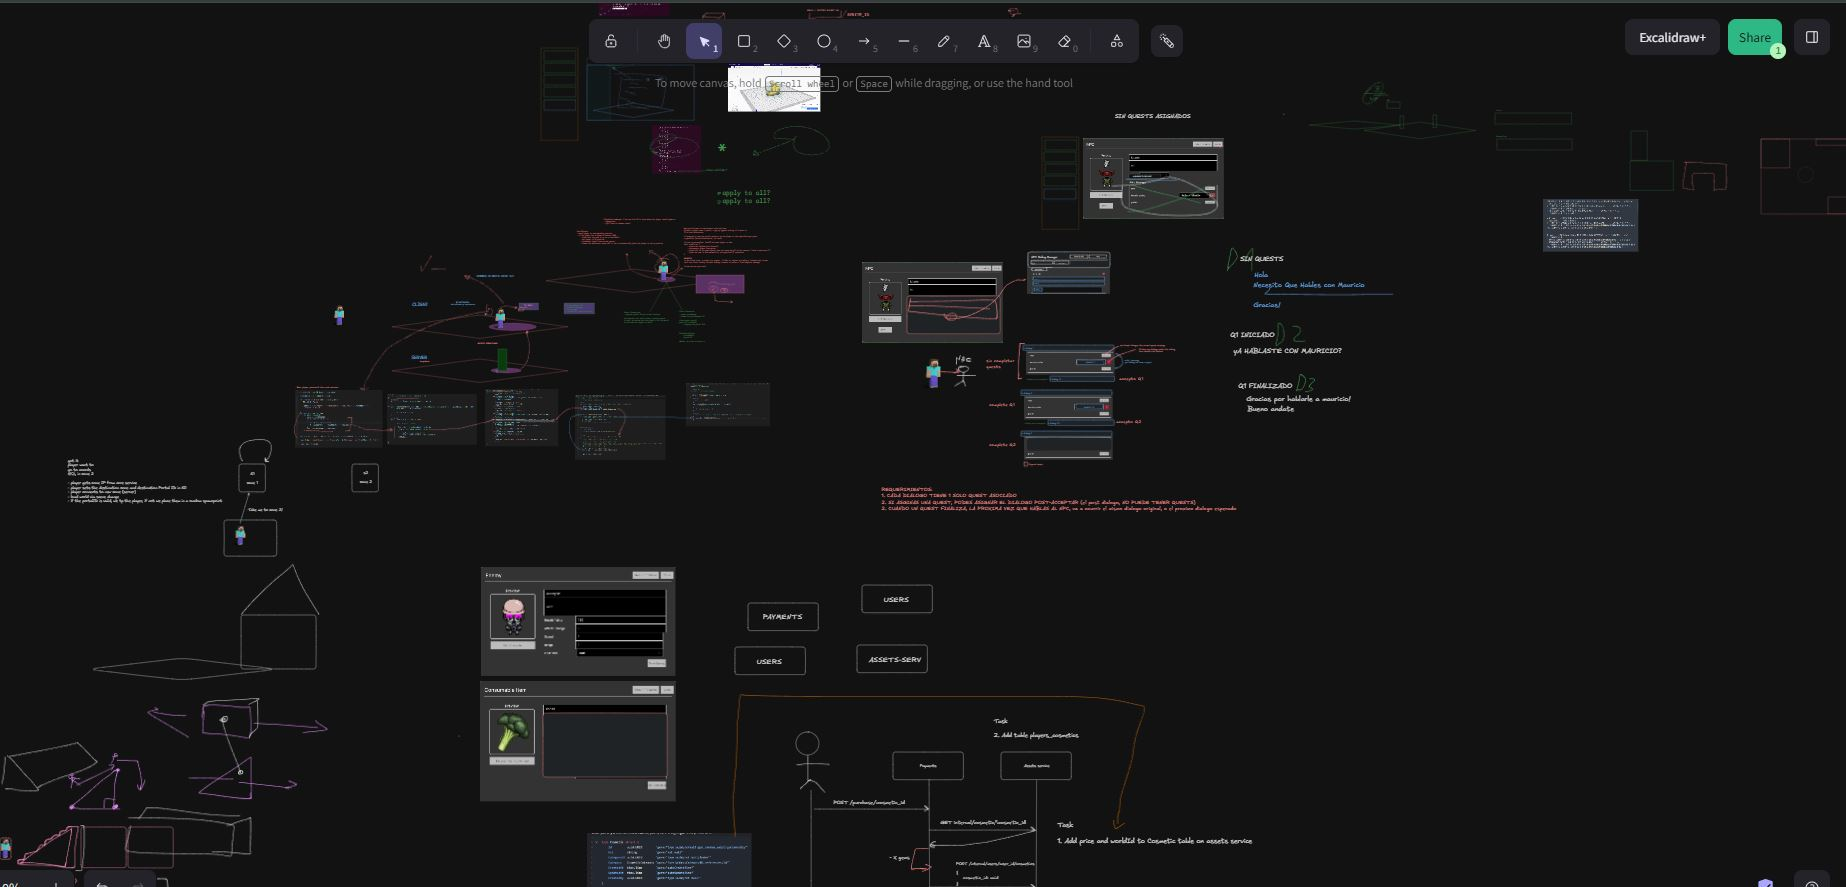
\includegraphics[width=0.85\textwidth]{img/excalidraw.jpg}
    \caption{Captura de brainstorming y croquis en Excalidraw.}
    \label{fig:excalidraw}
\end{figure}

\textbf{\underline{Discord}}: para compartir guías, tareas pendientes, información de spikes, comandos relevantes para 
ejecuciones y variables de entorno locales o temporales para comunicar cambios en entorno de desarrollo de los distintos 
sistemas del proyecto.
\vspace{0.25cm}

\begin{figure}[H]
    \centering
    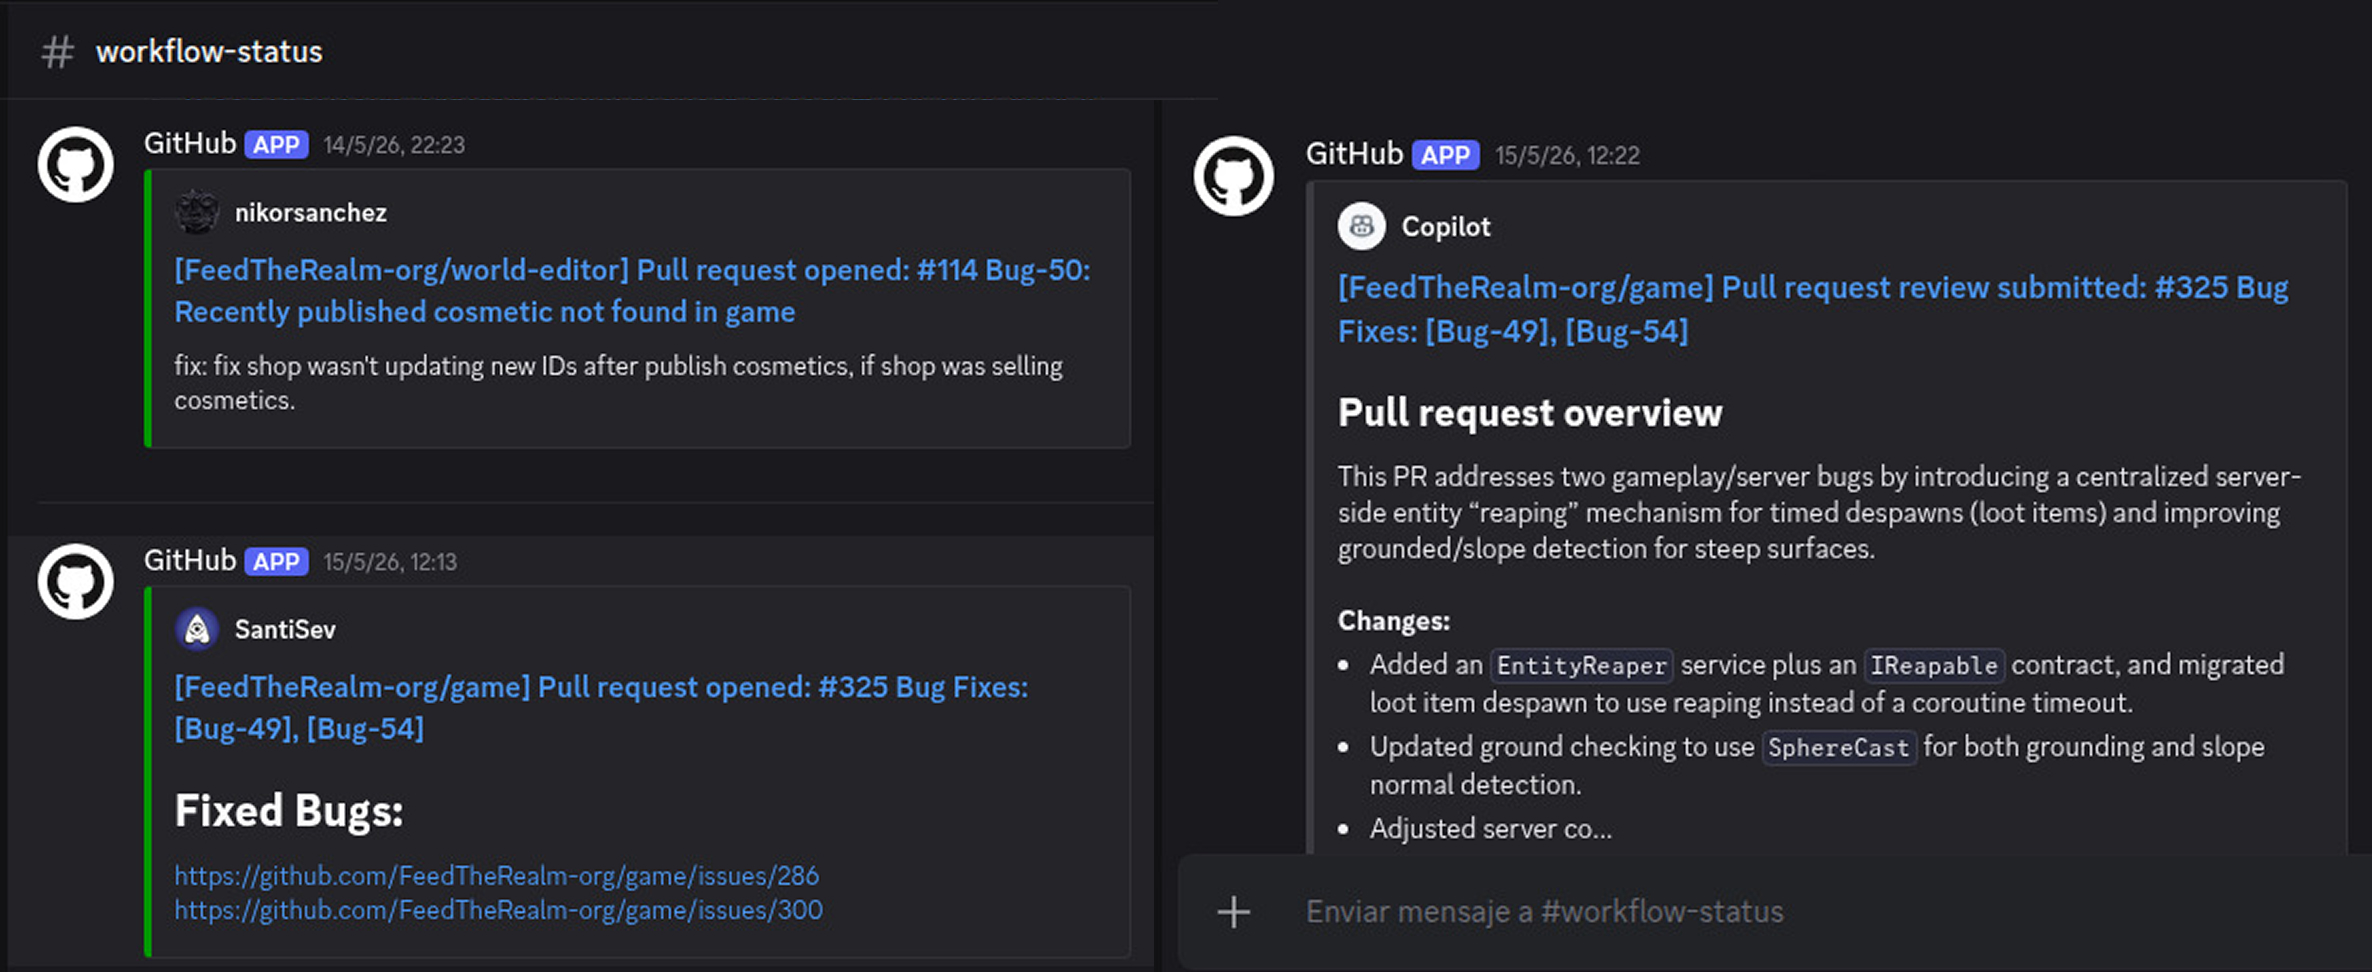
\includegraphics[width=0.85\textwidth]{img/discord.jpg}
    \caption{\textit{Screenshot} de Discord, herramienta utilizada para comunicación rápida y compartir información relevante.}
    \label{fig:discord}
\end{figure}

Relacionado a estas metodologías que se utilizó como herramienta degestión, se estableció ya desde el principio de desarrollo del proyecto, 
que deben haber 3 reuniones semanales fijas en cierto horario, generalmente a las 14hrs los dias lunes, miercoles y viernes, 
con el fin de actualizar los avances de todos los integrantes del grupo, hacer consenso de decisiones de diseño en las 
diferentes US y hacer tareas de planificación como se ha nombrado antes en fechas de comienzo/fin de iteración y 
comienzo/fin de nueva versión.
\vspace{0.25cm}

Por lo general se define un solo asignado a cada user story pero hubo casos donde se requirió suplantar al asignado 
principal por diferentes motivos que no pudo continuar, o se agregó un asignado más ya sea por una dificultad inesperada 
o que otra US quedó parcialmente acoplada/relacionada a la dicha. La metodología implementada en todos los casos con la 
salvedad en alguna excepción de prioridades en las US, tomar una US implicaría que el asignado a ella debe implementar 
todas las características que se requieran en los distintos servicios para que esté correctamente funcionando. Se tomó
la decisión que por tema de seguridad la regla de que un pull request antes de ser completado debe ser probado 
por otro integrante del grupo que no sea el asignado a la US relacionada, ya que la herramienta de Unity al 
versionar sus archivos pueden generar incongruencias o errores y puede llegar a no funcionar sin las 
configuraciones locales del integrante asignado, por distintos motivos.
\vspace{0.25cm}

\subsection{Gestión de iteraciones y versiones}

Como se mencionó anteriormente, se ha separado cada versión con duración de aproximadamente un mes, para poder tener 
parámetros del estado del proyecto a lo largo del tiempo y poder establecer un avance de él de forma incremental, 
ya que hay US que son dependientes una de otras y deben realizarse en cierto orden. Además, cada versión contiene 
dos iteraciones, cada una de dos semanas de duración aproximadamente. Ocasionalmente, se llegó a extender la duración debido a 
problemas de demora general del equipo por distintas cuestiones, como las otras materias cursadas en paralelo al proyecto, o 
que múltiples US esté casi por desplegarse y/o terminar de probar su integración.
\vspace{0.25cm}

La herramienta principal utilizada para reflejar el progreso más actualizado día a día fue Github Projects. Por lo tanto 
si se detecta algún \textit{bug} relacionado a una US fuera de su etapa de desarrollo por lo general se informa informalmente 
al asignado de ella en las reuniones. En el caso que involucre un cambio complejo su solución o se requiere registrar como 
replicar el \textit{bug}, se crea un ticket en esta plataforma para ser solucionado dentro de la iteración o para la etapa final 
de solución de \textit{bugs} y pulido de features y UI, dependiendo de la gravedad del \textit{bug}, si es necesario mitigar 
riesgos o si ese \textit{bug} puede afectar otra US y desencadenar fallas difíciles de detectar.
\vspace{0.25cm}

Como se mencionó anteriormente se decidió que las últimas dos iteraciones del total de ellas, sean destinadas a la última 
etapa de pulir últimos cambios y desarrollo de informe. Con últimos cambios se infiere a soluciones de \textit{bugs} 
pendientes, desarrollar aspectos a mejorar que en su momento se obviaron para tener US con funcionalidad suficiente, mejoras 
en la UI pendientes o para perfeccionar, features opcionales que mejoran la jugabilidad de los clientes y optimizaciones 
importantes para mejorar el rendimiento ya sea de los clientes como de los servidores.

\vspace{0.25cm}

Queda a aclarar que todas las US que fueron limitadas en su alcance fueron o diagramadas de tal forma previamente al 
momento de crear los CA al comienzo de iteración, o en las reuniones al ver qué la dificultad de la US fue subestimada 
y/o se extendió mucho la entrega completa de tal US con respecto a los tiempos de la iteración. Entonces o bien se crea 
una nueva US con las características a desarrollar pendientes en la próxima iteración o se crea una US para asignarse en 
la última etapa del proyecto.

\vspace{0.25cm}

Con respecto a las etapas del proyecto, se organizaron de forma de que para la entrega intermedia se tenga algunas o las 
mayorías características principales del proyecto funcionando y también la mayor parte de lo pactado con el tutor y lo 
escrito en la propuesta entregada antes de comenzar el proyecto. Se podría decir que logró un buen resultado con la gestión 
implementada, ya que se llegó a la etapa final con todas las características y funcionalidades principales esperadas 
completadas. Y además las US desestimadas no fueron en general features determinantes o muy relevantes con respecto a 
las realizadas sino más bien extras o complementarias.

\vspace{0.25cm}

\subsection{Métricas de planificación y gestión}

A continuación se mostrará las métricas obtenidas al final del proyecto, con el fin de analizar la planificación 
y gestión del mismo a lo largo del tiempo.

Para comenzar, se muestra la evolución del backlog a lo largo de las iteraciones, se contabiliza en el eje vertical 
la cantidad de US, y en el eje horizontal las iteraciones. 
Se puede observar que a lo largo del tiempo se mantuvo una cantidad desarrollada relativamente estable, 
con un pico sobre el final del proyecto, debido a que se agregaron US para mejorar/arreglar características ya 
desarrolladas o para agregar nuevas features complementarias y de diseño, lo cuales contaron con una mayor cantidad de US 
desarrolladas pero de menor complejidad y tiempo empleado para completarlas.

\begin{figure}[H]
    \centering
    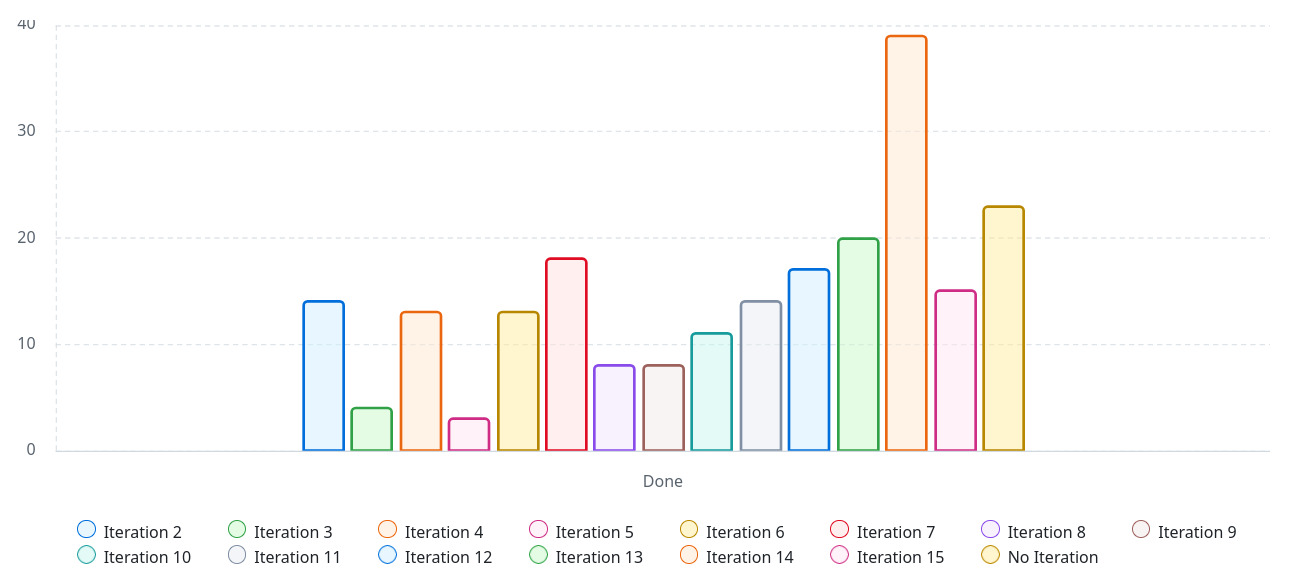
\includegraphics[width=0.85\textwidth]{img/09-applied-methology/backlog-iteration.jpg}
    \caption{Evolución del backlog a lo largo de las iteraciones.}
    \label{fig:backlog-iteration}
\end{figure}

En la siguiente gráfica se muestra la evolución del backlog a lo largo de las versiones, se contabiliza en el eje vertical
la cantidad de US, y en el eje horizontal las versiones. Se observa caraterísticas similares a la gráfica anterior, 
por la misma razón explicada anteriormente.

\begin{figure}[H]
    \centering
    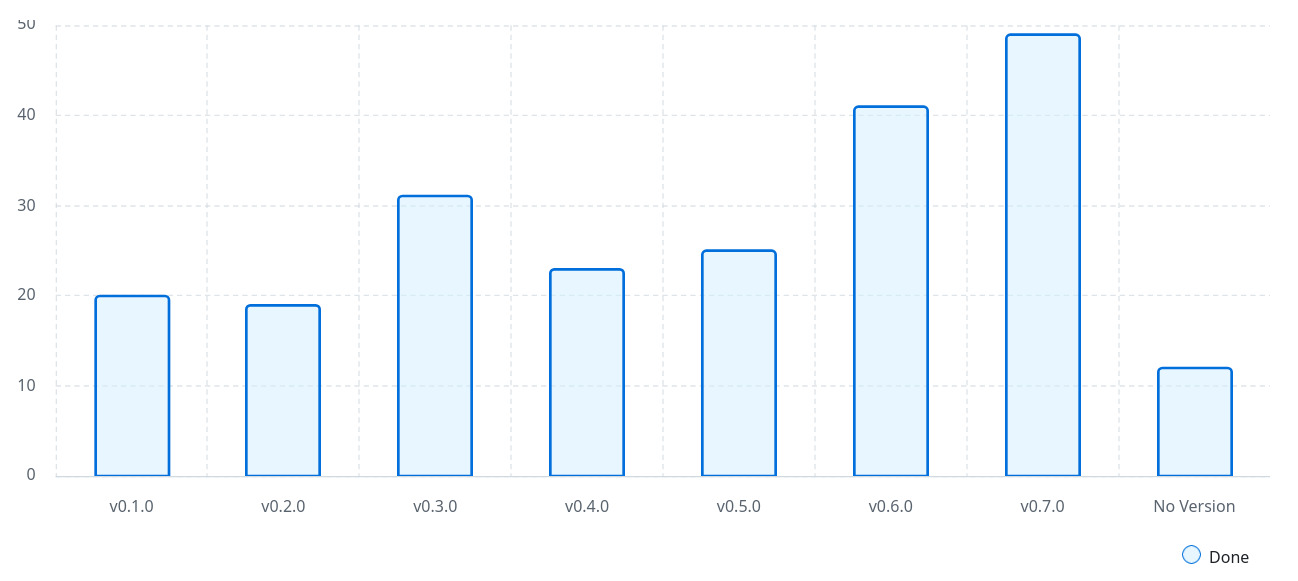
\includegraphics[width=0.85\textwidth]{img/09-applied-methology/backlog-version.jpg}
    \caption{Evolución del backlog a lo largo de las versiones.}
    \label{fig:backlog-version}
\end{figure}


Luego en esta gráfica se muestra la división de tareas por integrante del grupo en el proyecto, se contabiliza 
en el eje vertical la cantidad de US, y en el eje horizontal los integrantes del grupo. 
Se puede observar que la distribución de las US fue relativamente equitativa entre los integrantes, 
a pesar de verse distinciones en la cantidad asignada a cada integrante en ciertas etapas, se debe a que algunas 
de ellas fueron más complejas que otras y el tiempo de desarrollo de cada una de ellas no fue el mismo, 
a pesar de ello la distribución fue equitativa.


\begin{figure}[H]
    \centering
    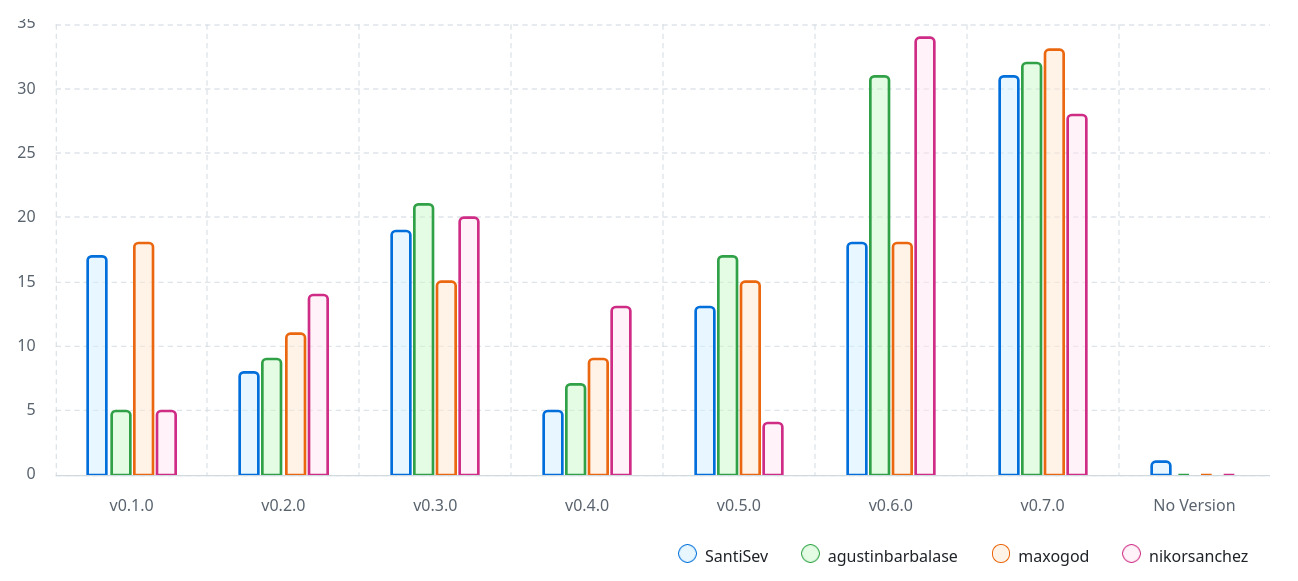
\includegraphics[width=0.85\textwidth]{img/09-applied-methology/team-division.jpg}
    \caption{Distribución de las US por integrante del grupo.}
    \label{fig:team-division}
\end{figure}


En cuanto a las US realizadas, se puede ver en el siguiente gráfico la distinción por tipo, se contabiliza en el 
eje vertical la cantidad, y en el eje horizontal sus tipos.


\begin{figure}[H]
    \centering
    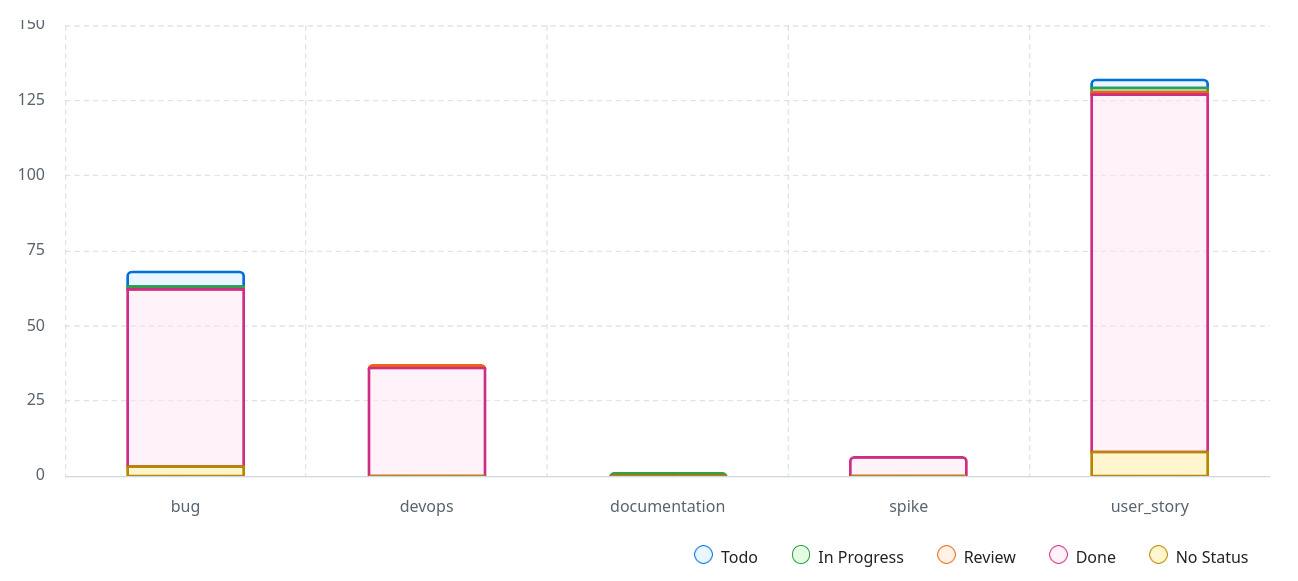
\includegraphics[width=0.85\textwidth]{img/09-applied-methology/labeled-status.jpg}
    \caption{Distribución de las US por tipo.}
    \label{fig:labeled-status}
\end{figure}


Con respecto a métricas de \textit{velocity}, se mostrarán a continuación dos gráficas. La primera se muestra con
respecto a la cantidad de US completadas por versión, se contabiliza en el eje vertical la cantidad de US, y 
en el eje horizontal las versiones. Se puede observar que a lo largo del proyecto se mantuvo una cantidad relativamente 
homogénea de US completadas por iteración, con un pico sobre el final del proyecto debido a lo ya explicado anteriormente 
sobre la acción en la última etapa.


\begin{figure}[H]
    \centering
    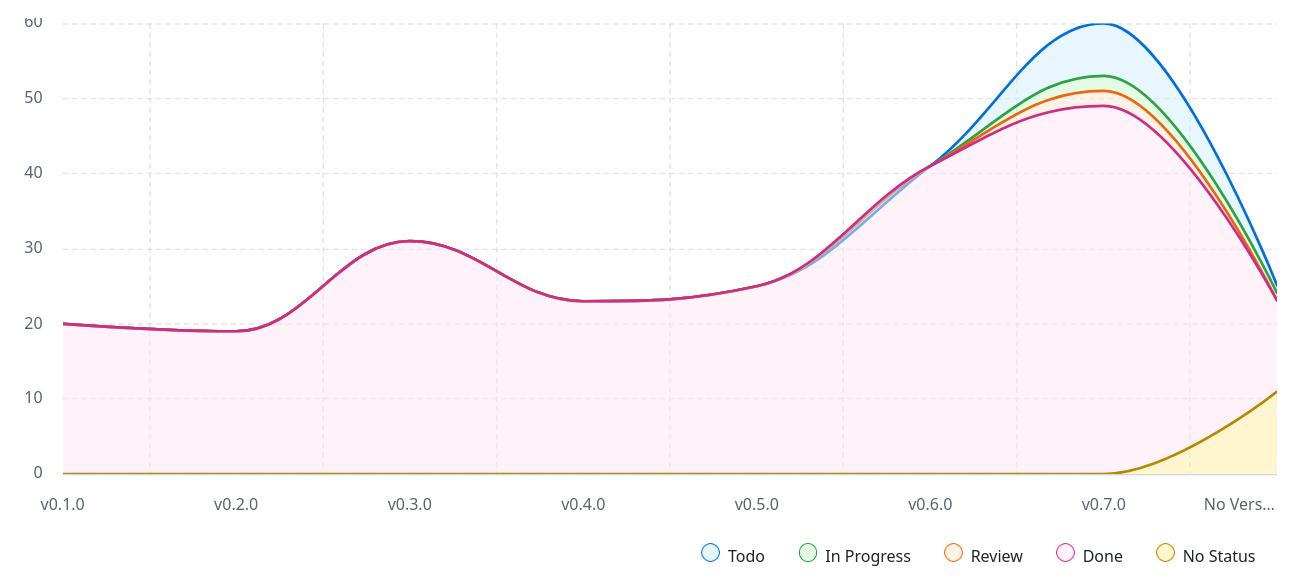
\includegraphics[width=0.85\textwidth]{img/09-applied-methology/velocity-tickets.jpg}
    \caption{Velocidad del equipo a lo largo de las versiones por cantidad de tickets.}
    \label{fig:velocity-tickets}
\end{figure}


Luego, se muestra la velocidad del equipo a lo largo de las versiones por puntos de estimación, propuestas en las reuniones 
de planificación de cada iteración utilizando la metodología de \textit{Planning Poker}, se contabiliza en el eje 
vertical la cantidad de puntos de estimación, y en el eje horizontal las versiones.


\begin{figure}[H]
    \centering
    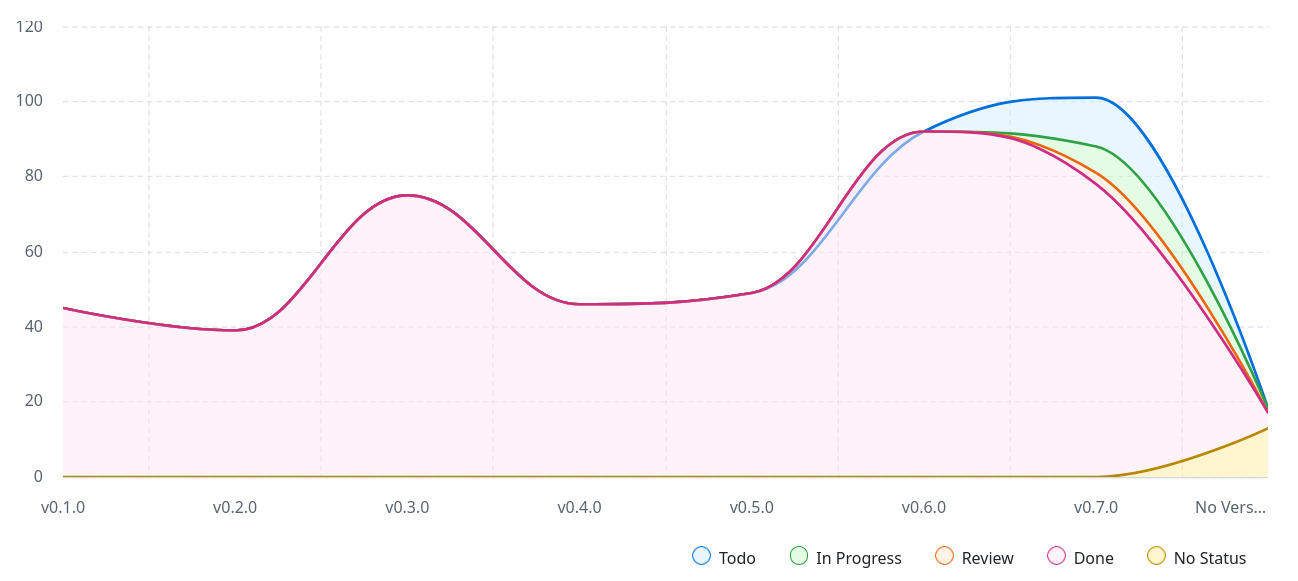
\includegraphics[width=0.85\textwidth]{img/09-applied-methology/velocity-estimate.jpg}
    \caption{Velocidad del equipo a lo largo de las versiones por puntos de estimación.}
    \label{fig:velocity-points}
\end{figure}


Por último, se puede observar en la siguiente gráfica el \textit{burn up} del proyecto, donde se contabiliza 
en el eje vertical la cantidad de US , y en el eje horizontal las fechas durante el proyecto en etapa de desarrollo. 
Se puede observar que a lo largo del proyecto se mantuvo una cantidad relativamente estable de US completadas en relación 
a lo que se planificaba tener realizado, como se explicó en esta sección, se hacía un analisis si se postergaba cada US 
a la siguiente iteración, o si se descartaba, y se puede observar en el gráfico que en determinada fecha a inicios de 
marzo, donde ya se planificaba el cierre de la etapa de desarrollo, que un número de US ya se determinaron como fuera del 
alcance del proyecto, y se decidió no desarrollarlas, lo cual se refleja en el gráfico como el incremento de US cerradas, 
y la brecha entre lo planificado y lo realizado se disminuye al llegar al fin.


\begin{figure}[H]
    \centering
    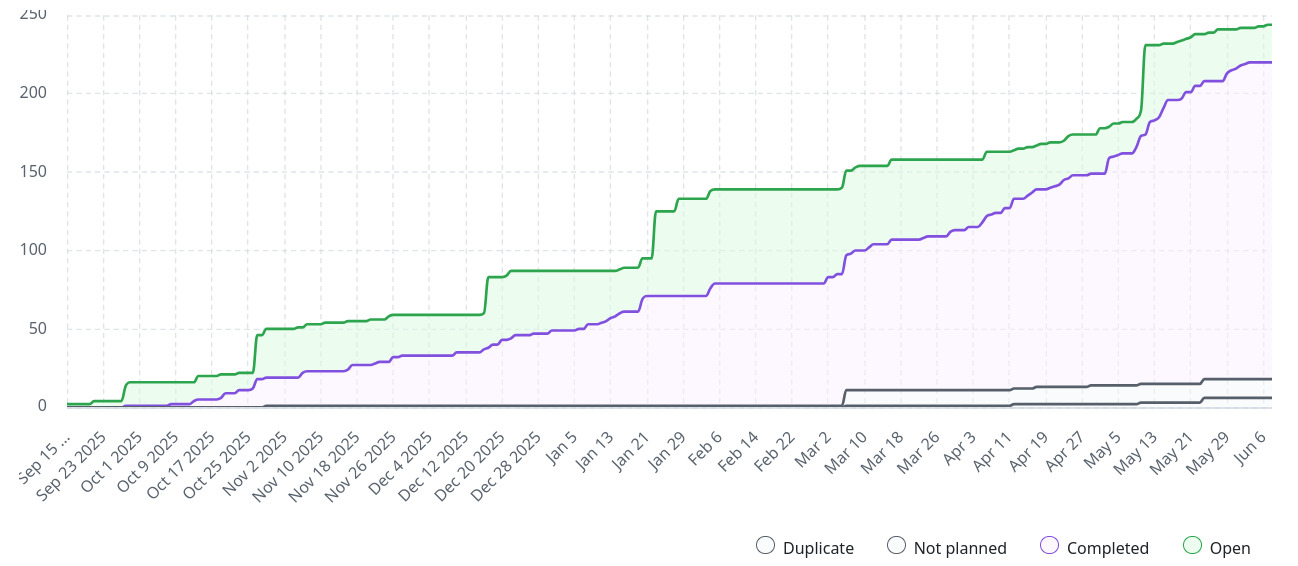
\includegraphics[width=1\textwidth]{img/09-applied-methology/burnup.jpg}
    \caption{Gráfico de \textit{burn up} del proyecto.}
    \label{fig:burnup}
\end{figure}

